\section{Algorithm evaluation}

    \subsection{Explanation}

        \begin{frame}
            \frametitle{EWC}
            \framesubtitle{Elastic Weight Consolidation}

            \begin{columns}[onlytextwidth]
                \column{.5\textwidth}
                    \begin{itemize}
                        \item protects previous \\gained knowledge
                        \item classifies importance \\of each thread
                        \item adaption of less important threads at re-training
                        \item protection discovery with Fisher Information matrix
                    \end{itemize}
                \column{.5\textwidth}
                \begin{figure}[H]
                    \centering
                    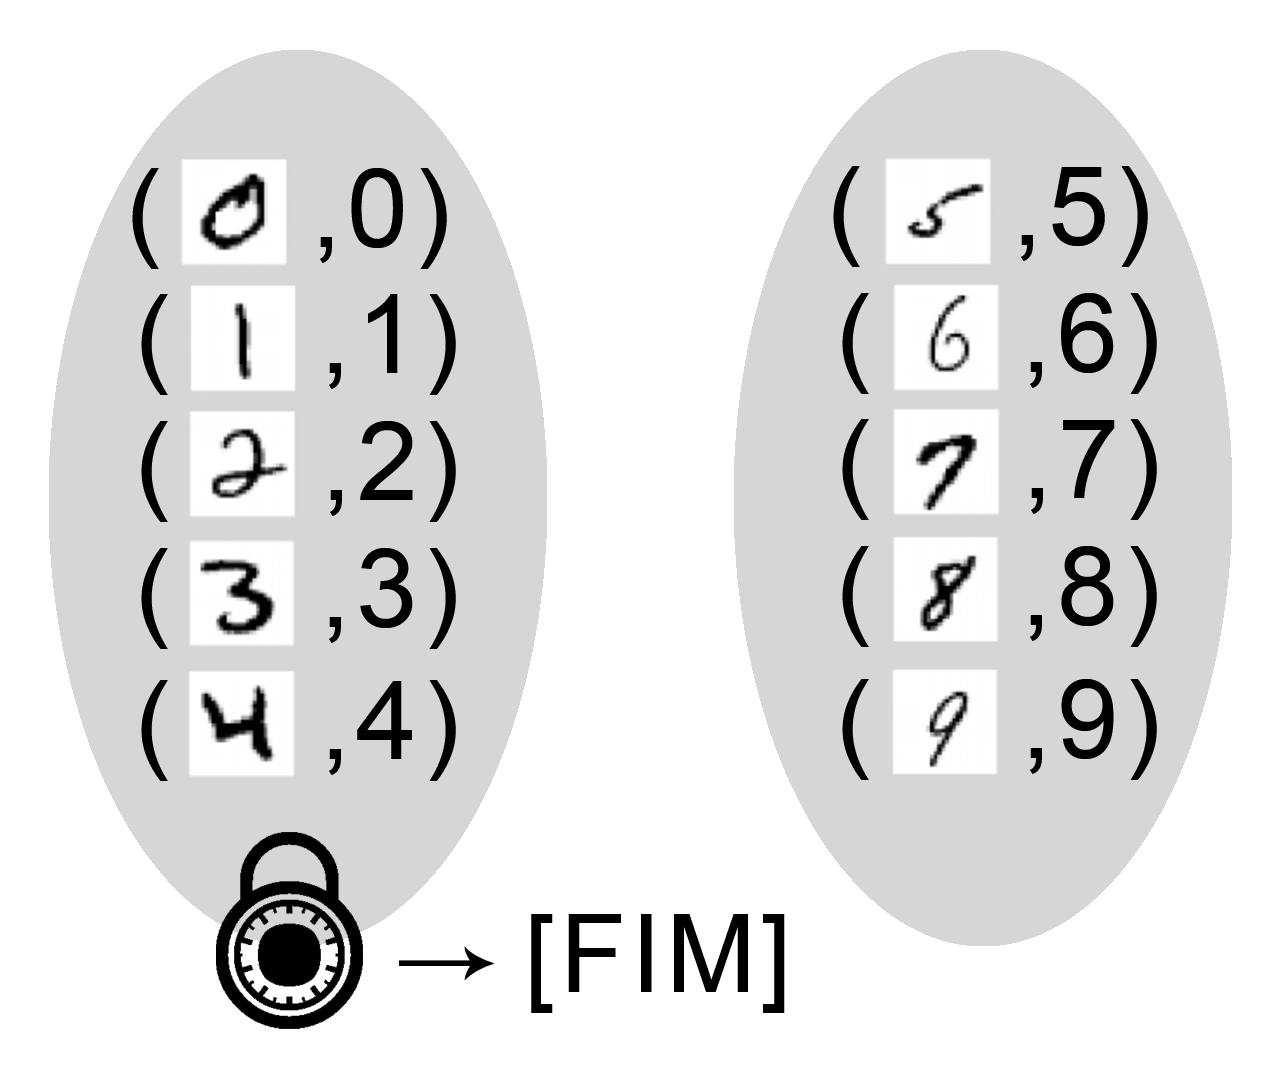
\includegraphics[width=\textwidth]{ewc}
                    \label{fig:ewc_expl}
                \end{figure}
            \end{columns}

        \end{frame}

    \subsection{Review \& Improvements}

        \begin{frame}
            \frametitle{EWC}
            \framesubtitle{Review}

            \begin{columns}[onlytextwidth]
                \column{.5\textwidth}
                    \begin{itemize}
                        \item unproven assumptions
                        \item implementation problem\\with TensorFlow
                    \end{itemize}
                \column{.5\textwidth}
                \begin{figure}[H]
                    \centering
                    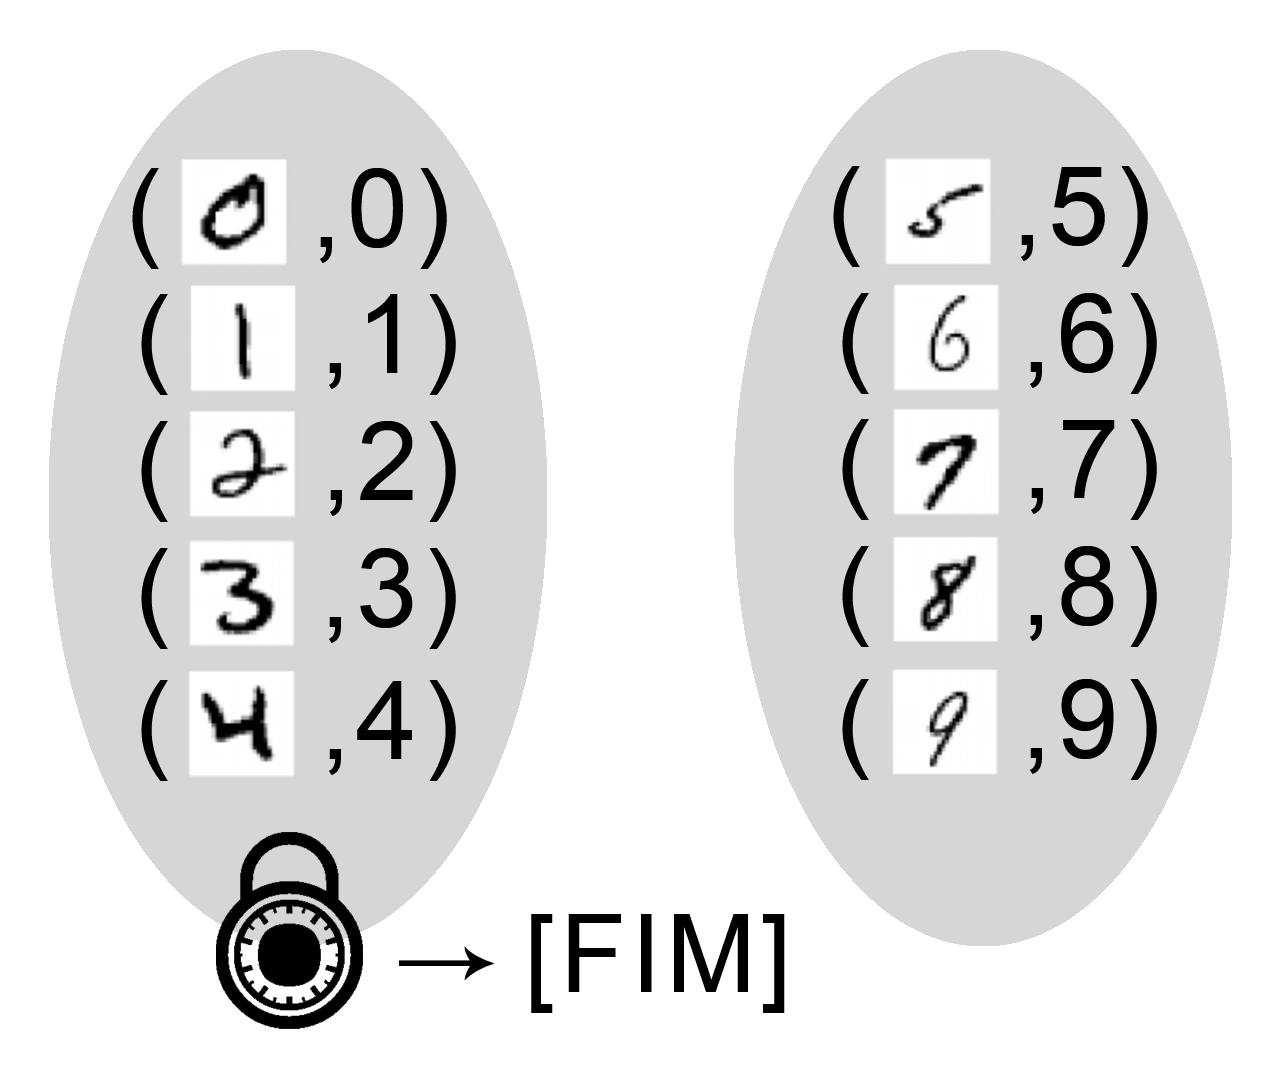
\includegraphics[width=\textwidth]{ewc}
                \end{figure}
            \end{columns}
        \end{frame}

        \begin{frame}
            \frametitle{EWC}
            \framesubtitle{Improvements}

            \begin{columns}[onlytextwidth]
                \column{.5\textwidth}
                    \begin{itemize}
                        \item replace FIM with new matrix (Gradient matrix)
                        \item less assumptions necessary
                        \item solves implementation problem in TensorFlow
                    \end{itemize}
                \column{.5\textwidth}
                \begin{figure}[H]
                    \centering
                    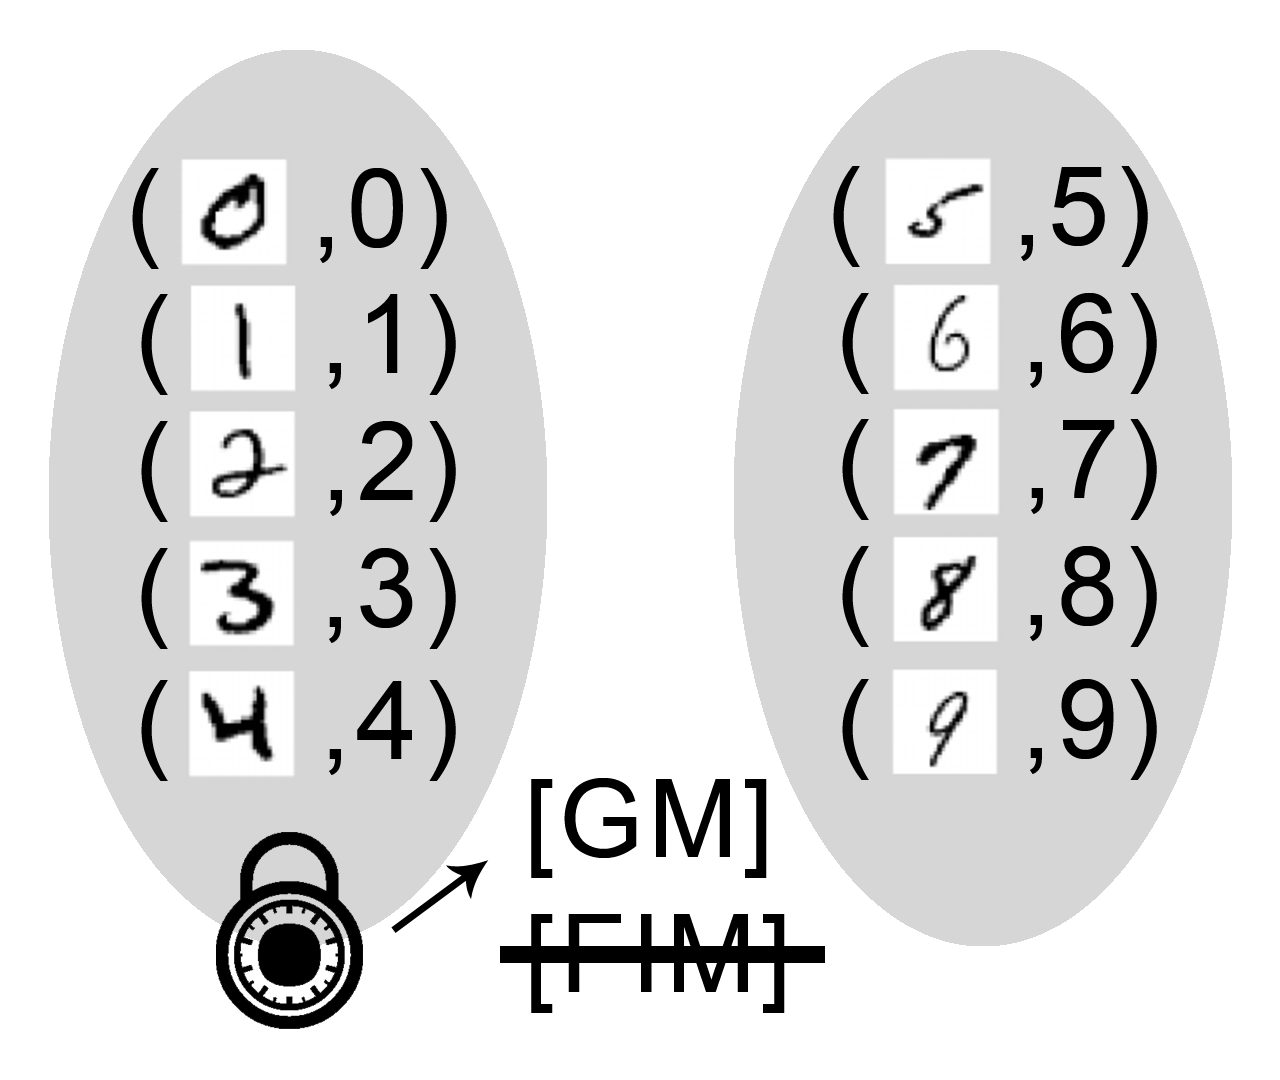
\includegraphics[width=\textwidth]{ewc_improvement}
                    \label{fig:ewc_improve}
                \end{figure}
            \end{columns}
        \end{frame}


    \subsection{Benchmarks}

        \begin{frame}
            \frametitle{Approach}

            \begin{figure}[H]
                \centering
                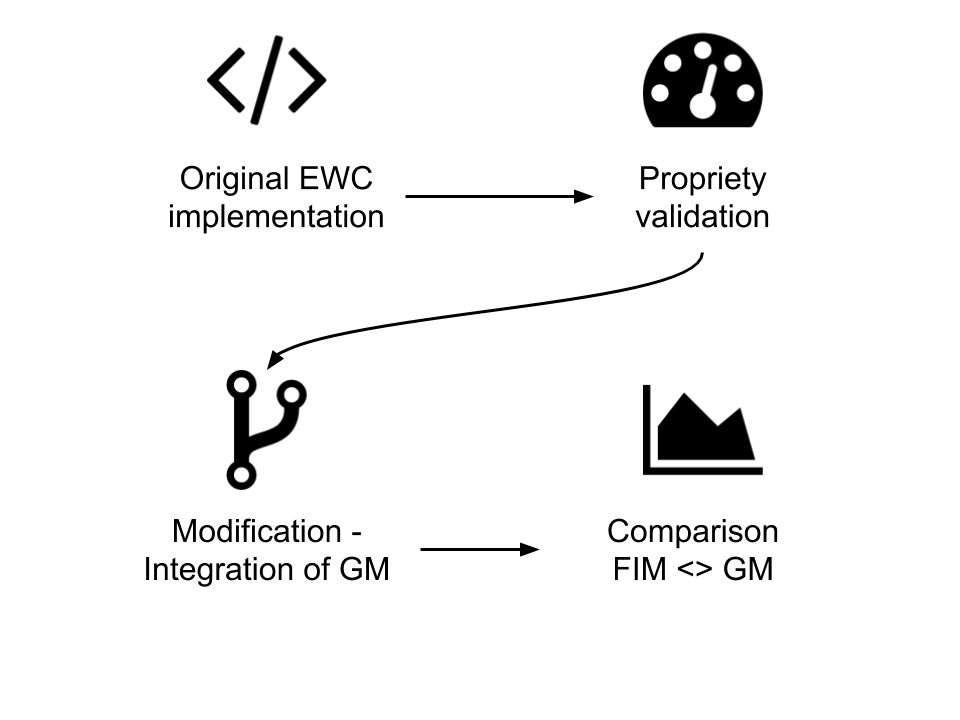
\includegraphics[width=\textwidth]{approach}
            \end{figure}

            % \begin{enumerate}
            %     \item Original EWC implementation
            %     \item Propriety validation
            %     \item Replacement of FIM with GM
            %     \item Comparison of modification and implementation
            % \end{enumerate}
        \end{frame}

        \begin{frame}
            \frametitle{Benchmark}
            \framesubtitle{Disjoint D9-1}

            \begin{itemize}
                \item T1: 9 classes; T2: 1 class
                \item discovers the capability of a re-training with small datasets
                \item approximately 10\% added
            \end{itemize}

            \begin{columns}
                \column{0.5\textwidth}
                \begin{figure}[H]
                    \centering
                    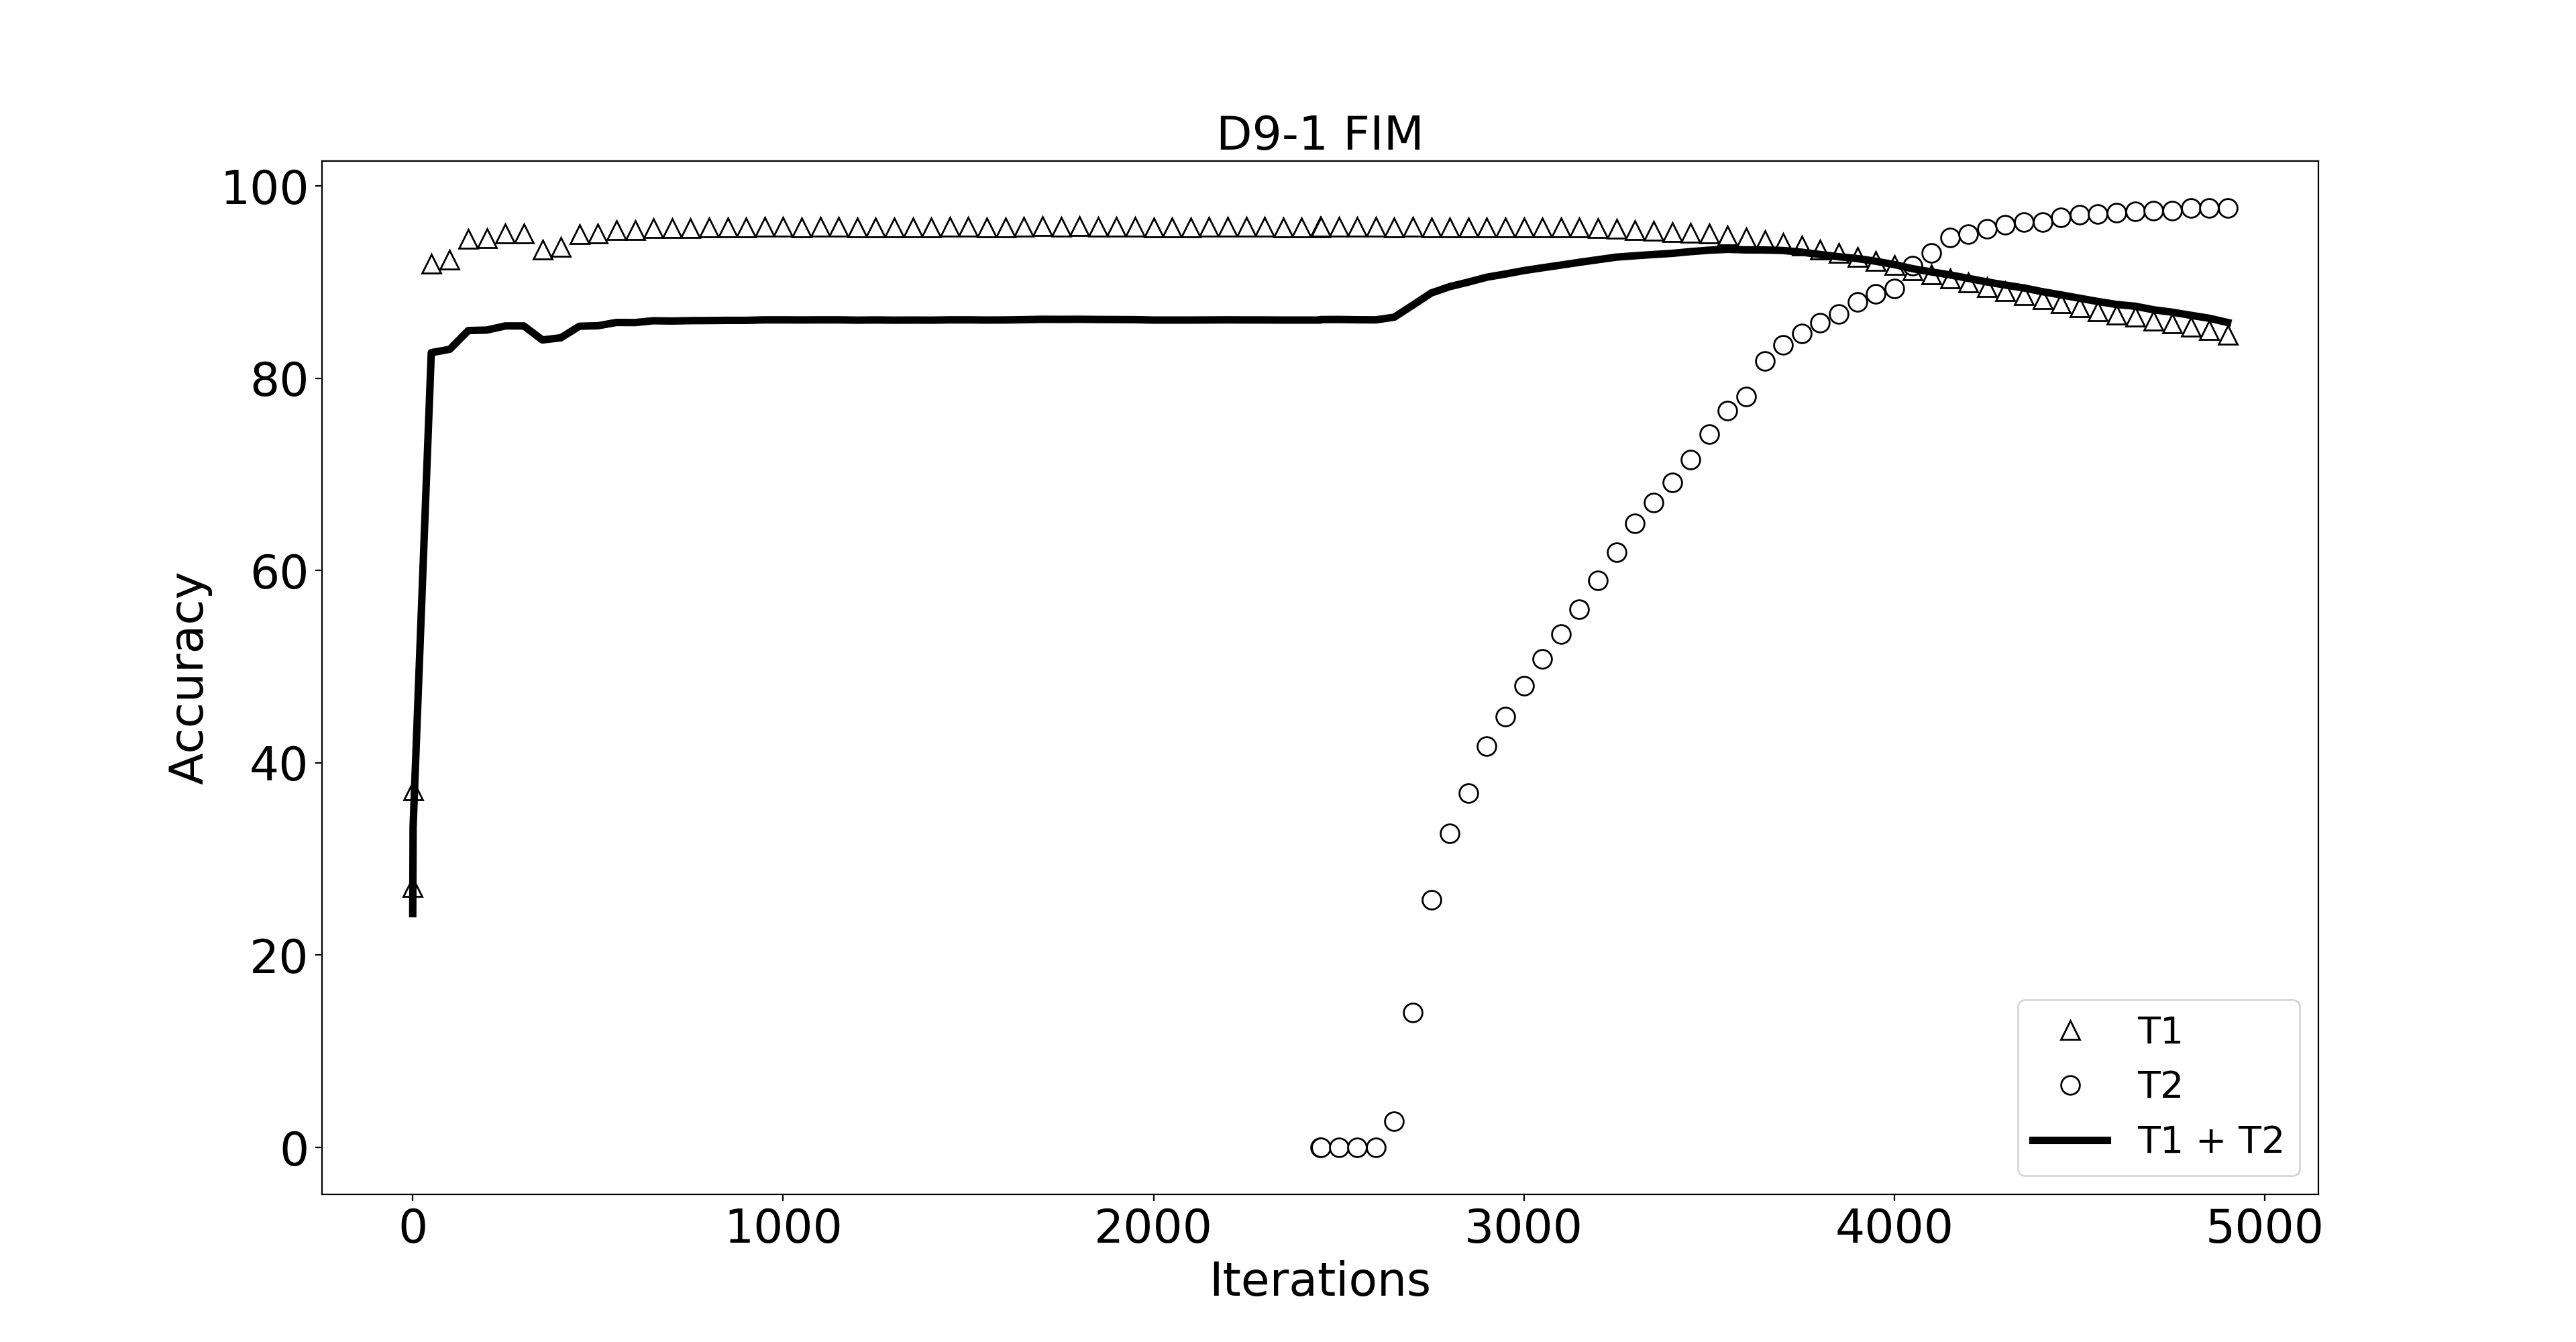
\includegraphics[width=\textwidth]{project/baseline/D91_FIM}
                    \caption{EWC-FIM D9-1}
                    \label{fig:ewc_fim_d91}
                \end{figure}
                \column{0.5\textwidth}
                \begin{figure}[H]
                    \centering
                    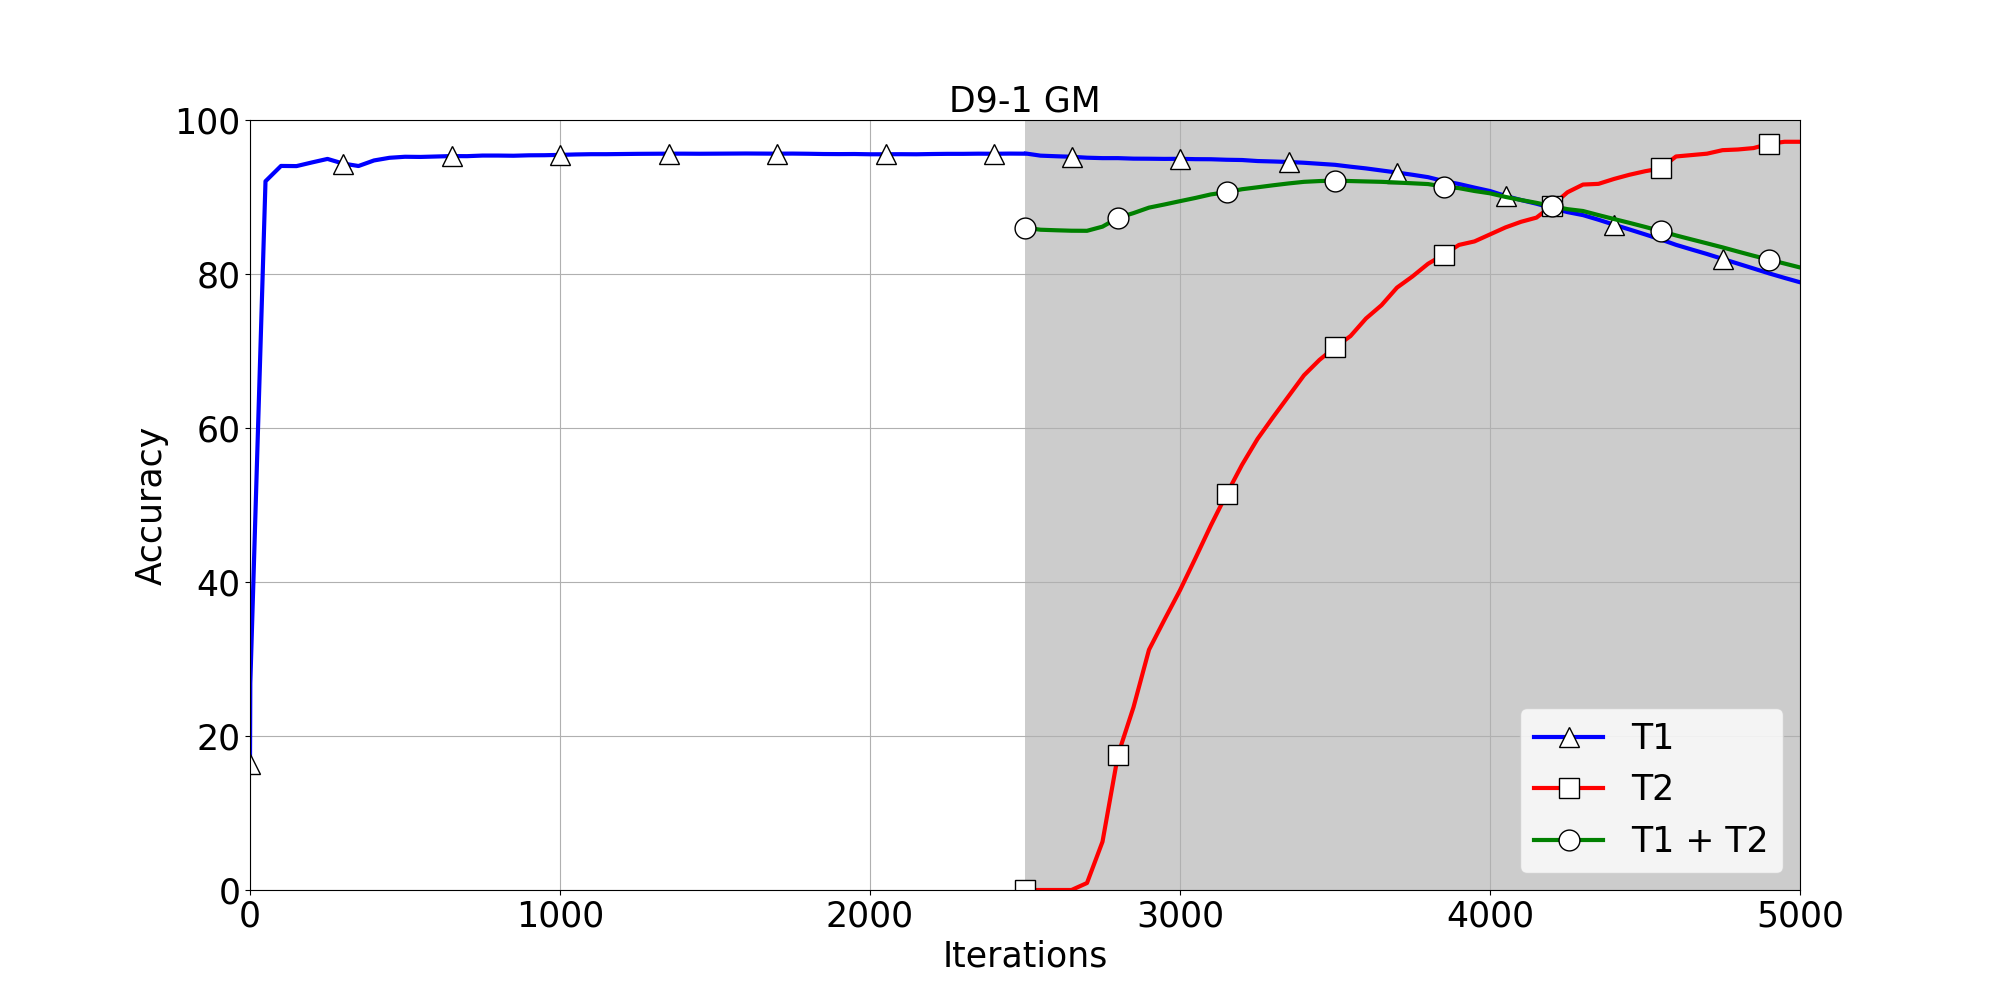
\includegraphics[width=\textwidth]{project/experiments/D91_GM}
                    \caption{EWC-GM D9-1}
                    \label{fig:ewc_gm_d91}
                \end{figure}
            \end{columns}
        \end{frame}

        \begin{frame}
            \frametitle{Benchmark}
            \framesubtitle{Disjoint D5-5}
            
            \begin{itemize}
                \item T1: 5 classes; T2: 5 classes
                \item challenge to handle the same data volume
            \end{itemize}

            \begin{columns}
                \column{0.5\textwidth}
                \begin{figure}[H]
                    \centering
                    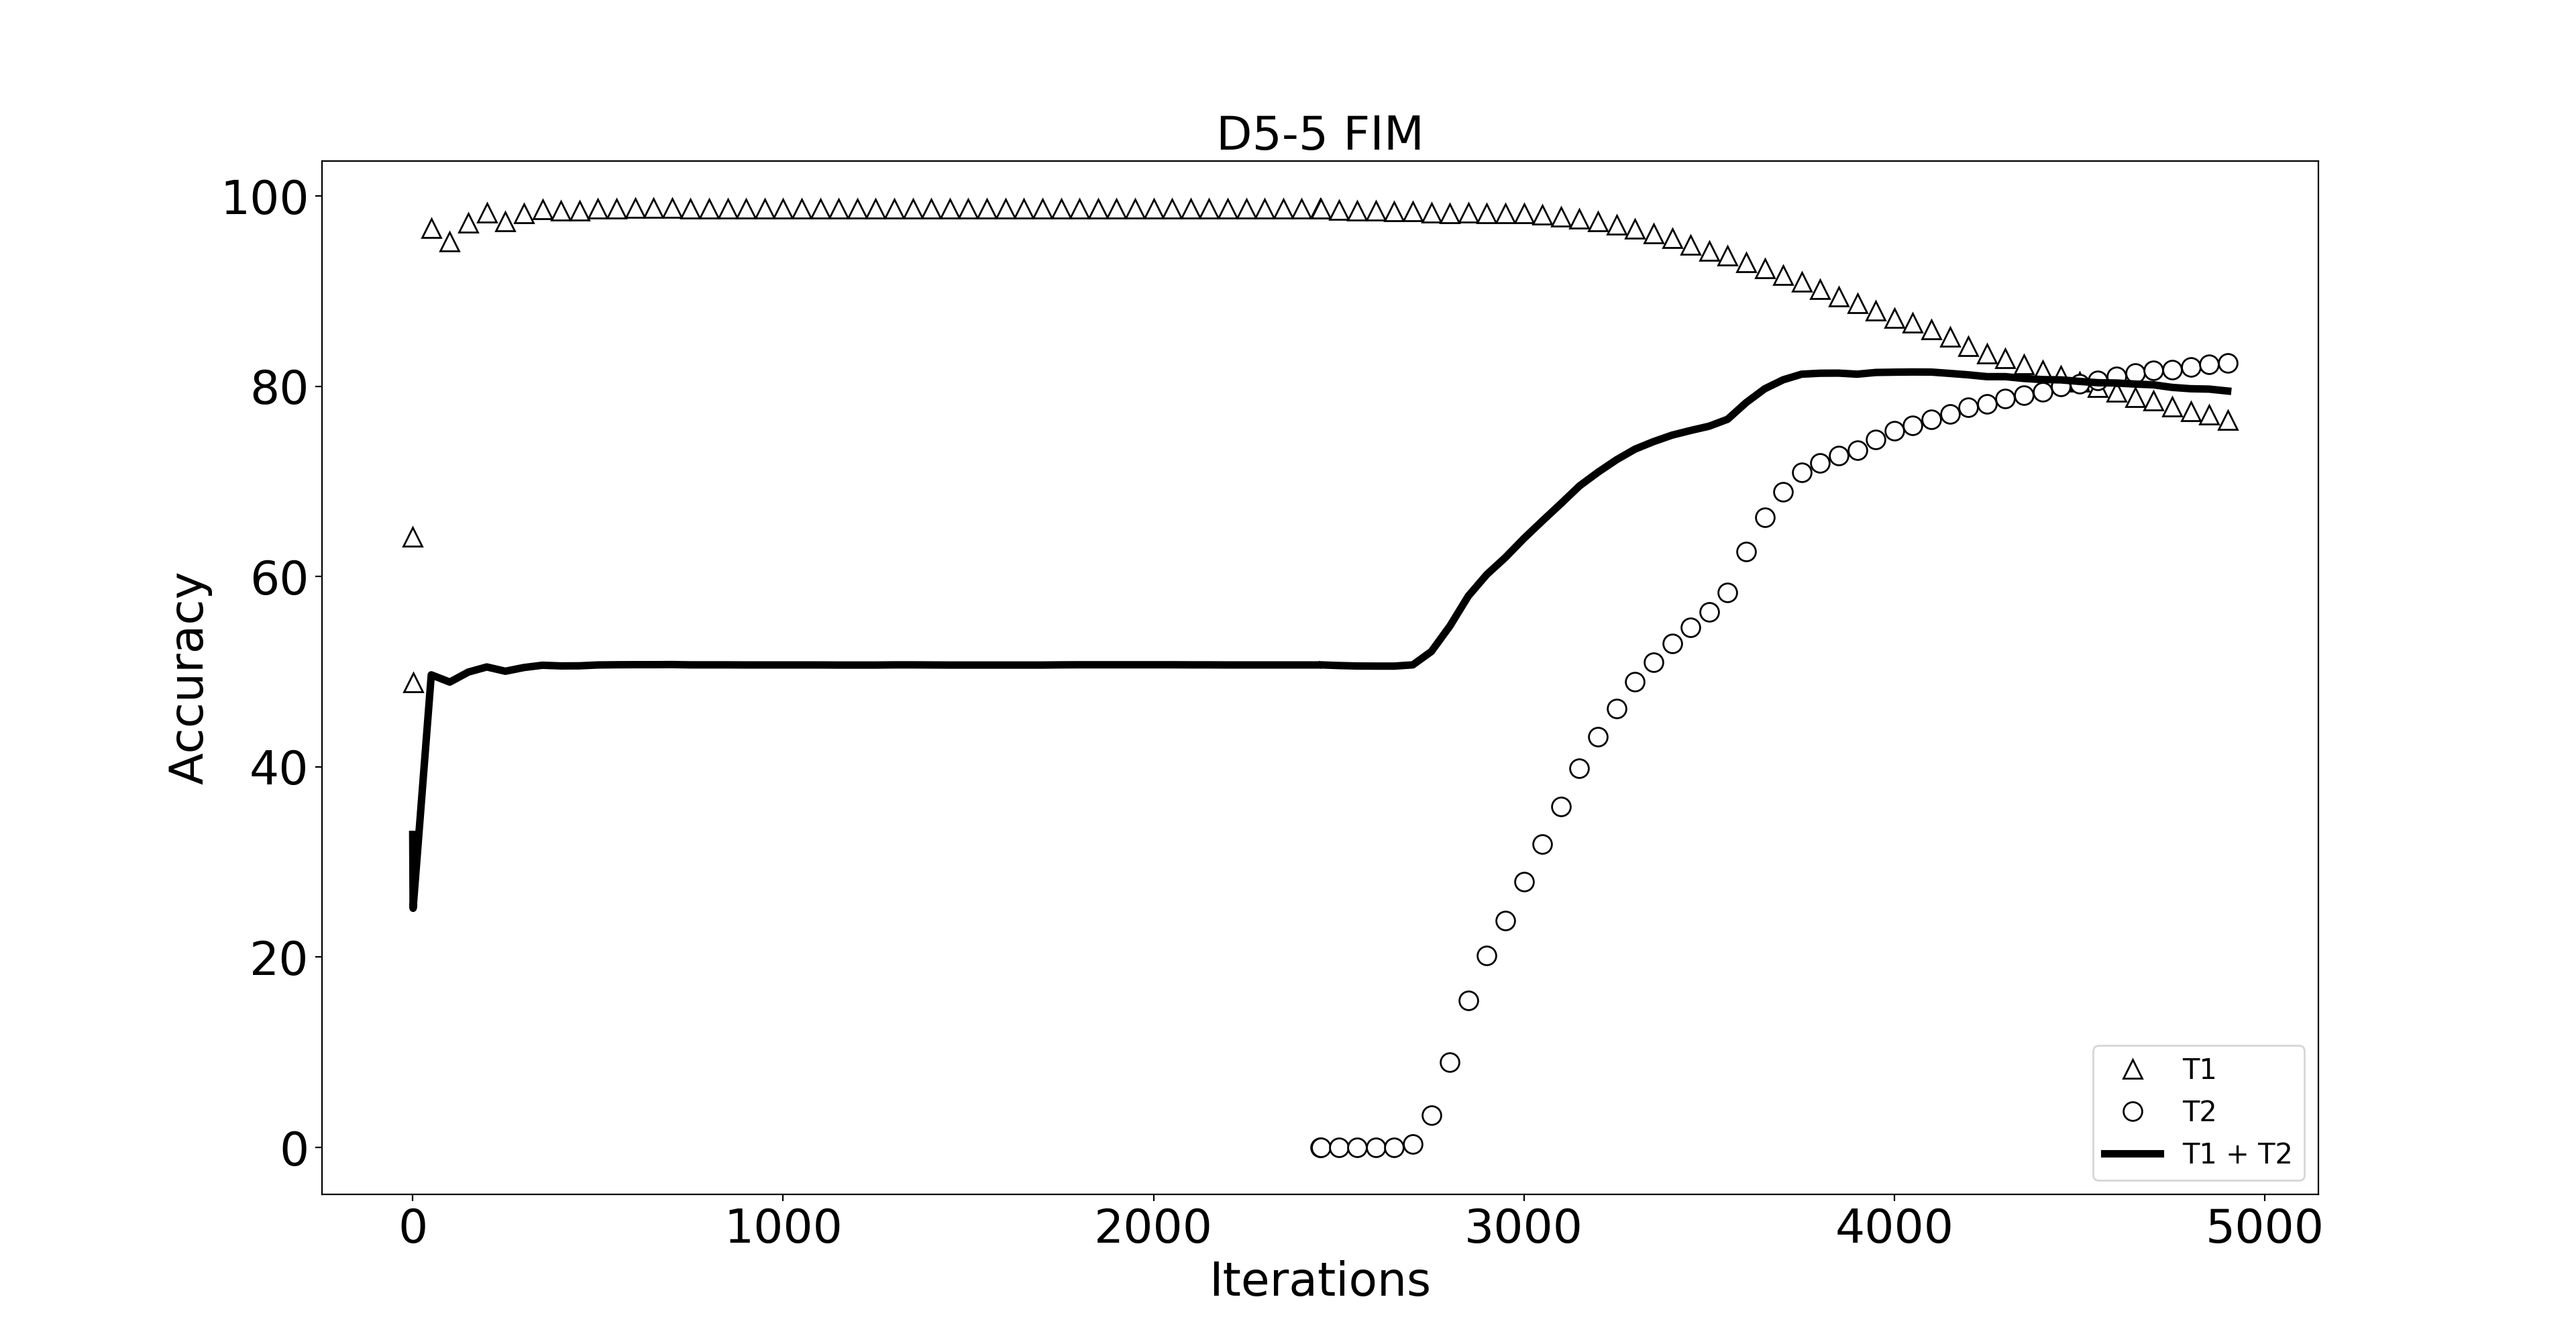
\includegraphics[width=\textwidth]{project/baseline/D55_FIM}
                    \caption{EWC-FIM D5-5}
                    \label{fig:ewc_fim_d55}
                \end{figure}
                \column{0.5\textwidth}
                \begin{figure}[H]
                    \centering
                    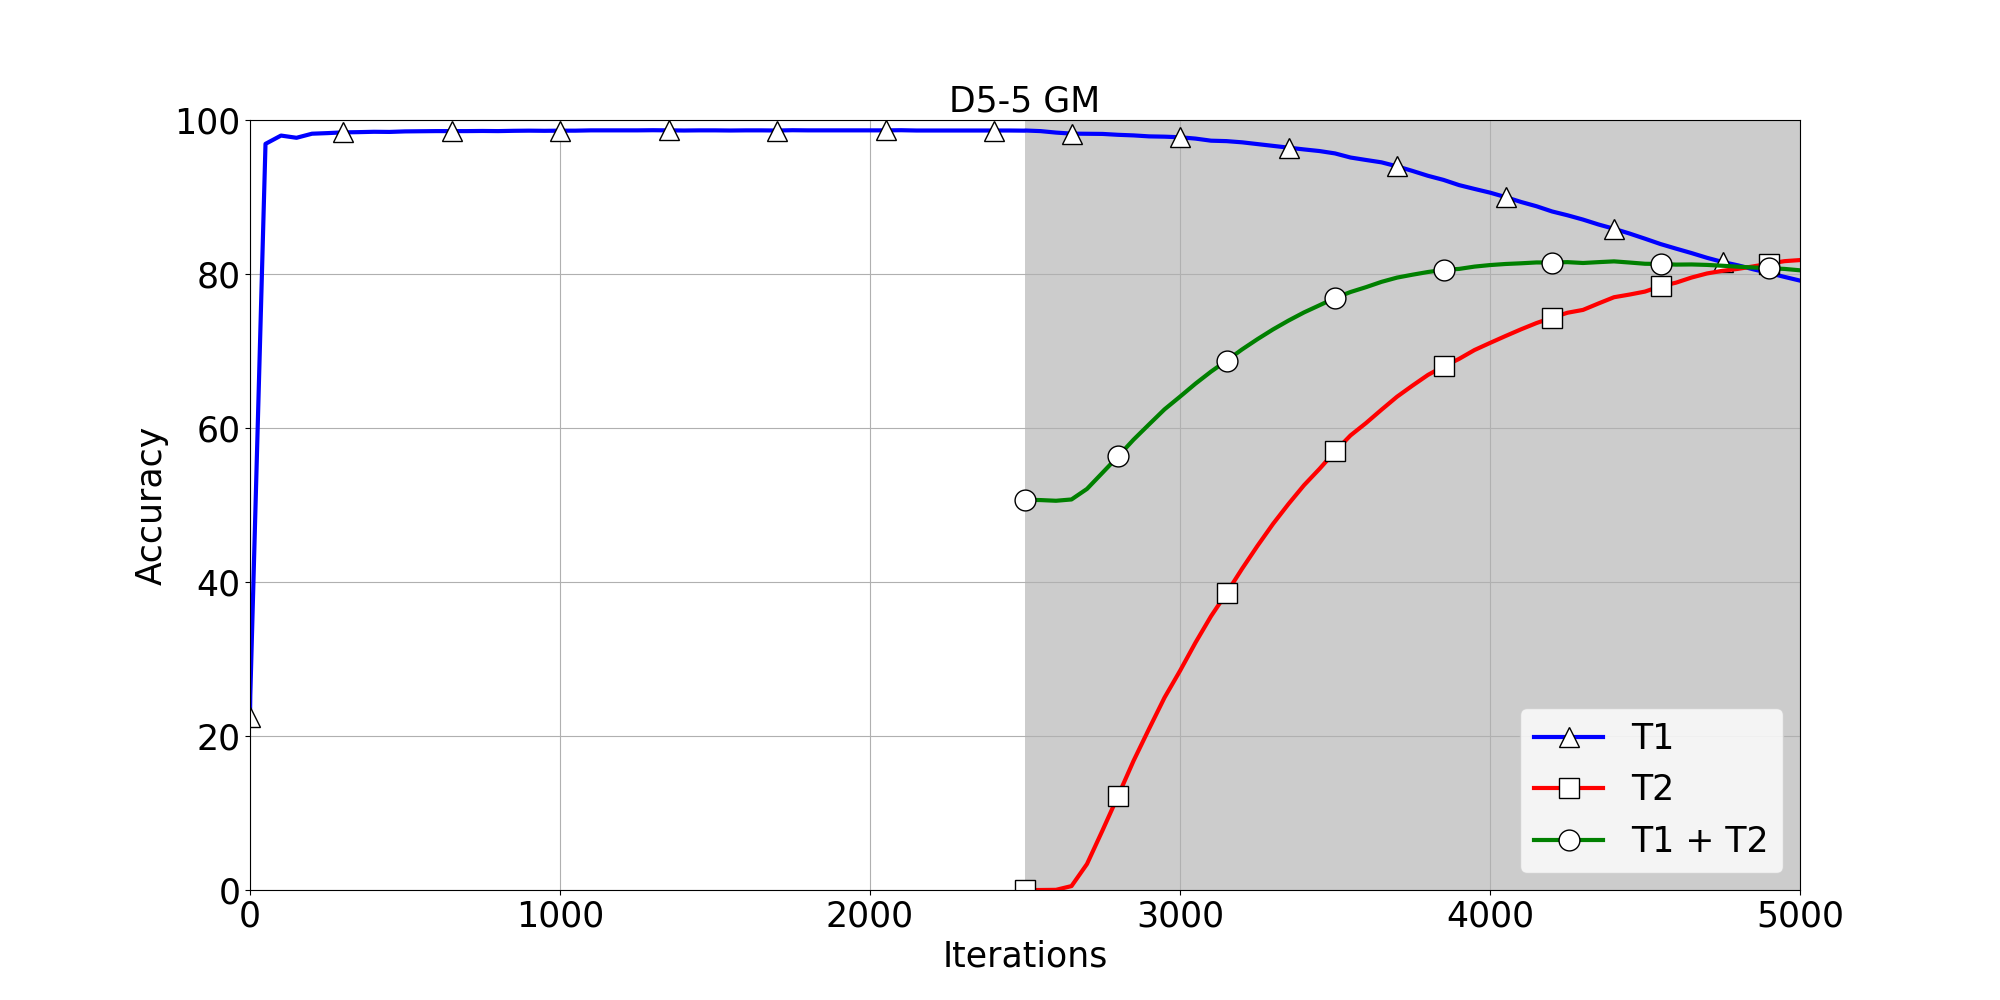
\includegraphics[width=\textwidth]{project/experiments/D55_GM}
                    \caption{EWC-GM D5-5}
                    \label{fig:ewc_gm_d55}
                \end{figure}
            \end{columns}
        \end{frame}

        \begin{frame}
            \frametitle{Benchmark}
            \framesubtitle{Permuted P10-10}

            \begin{itemize}
                \item T1: 10 classes; T2: permuted classes
                \item challenge to learn different data-chunks with the same classes
            \end{itemize}

            \begin{columns}
                \column{0.5\textwidth}
                \begin{figure}[H]
                    \centering
                    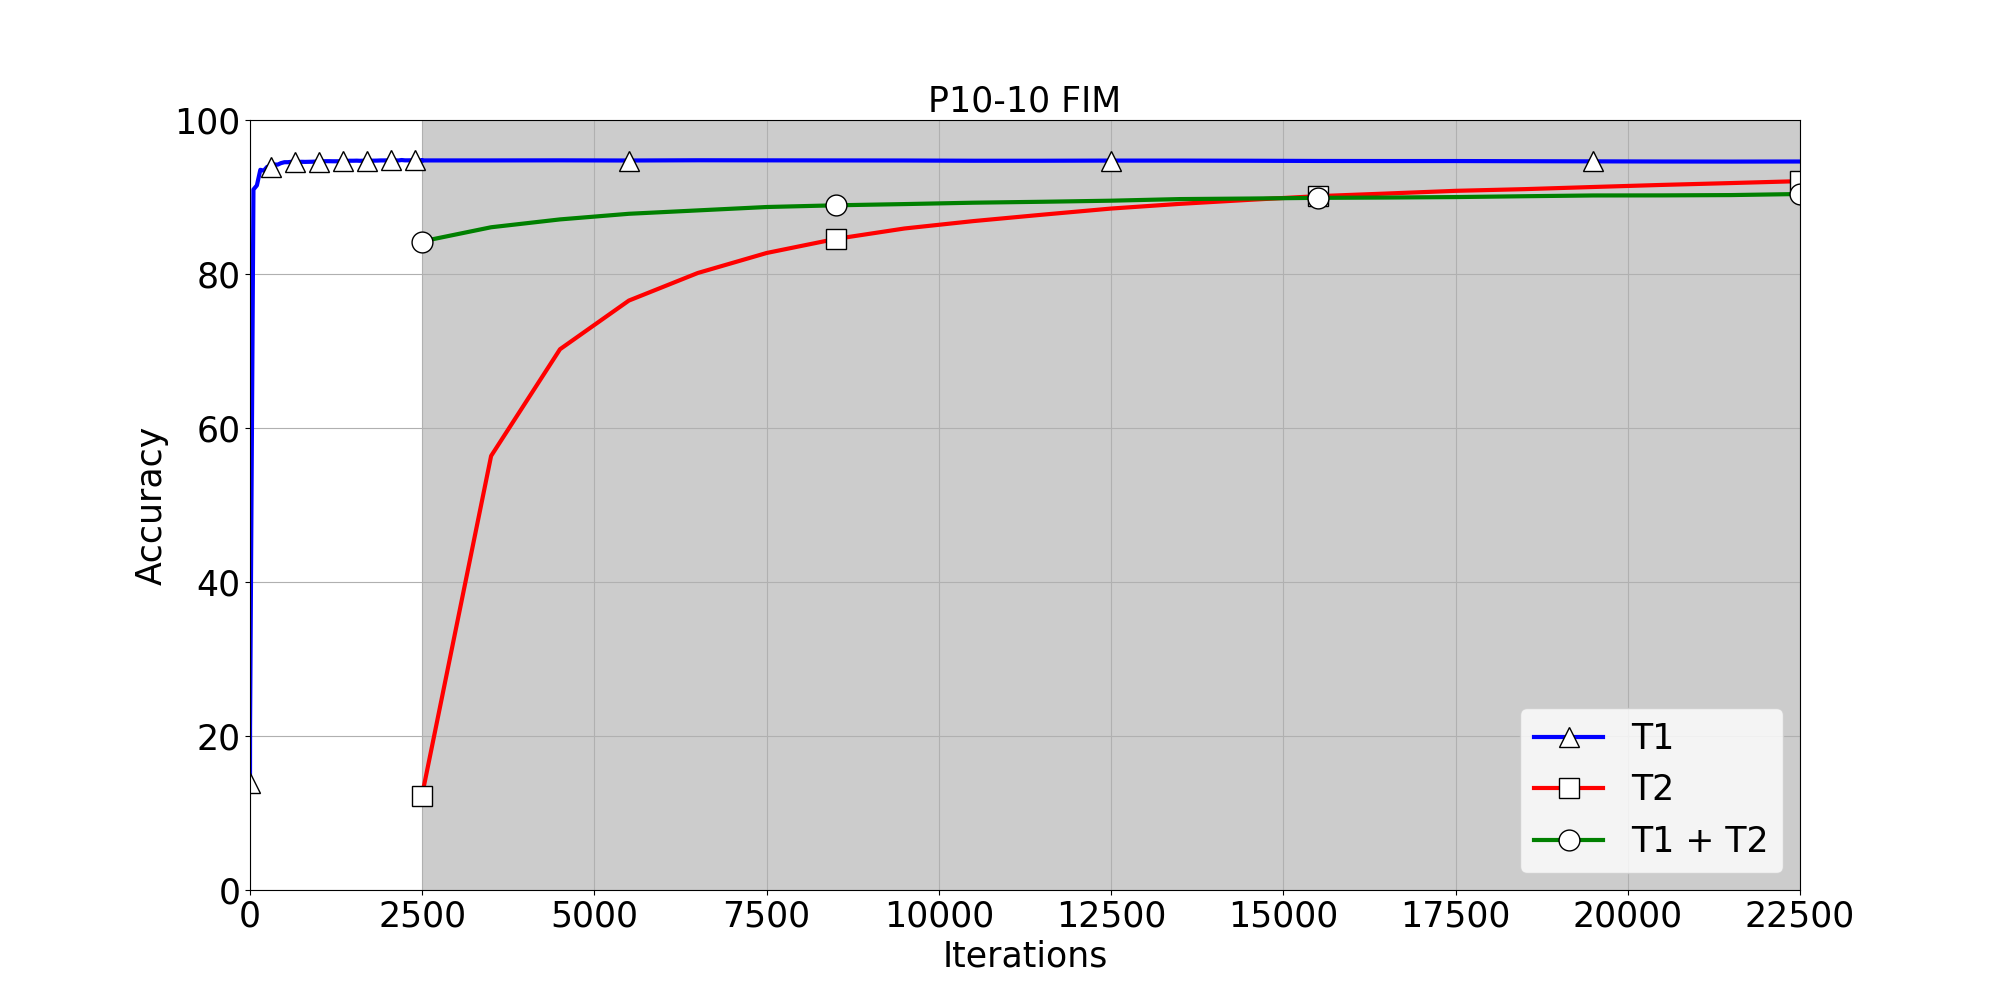
\includegraphics[width=\textwidth]{project/baseline/PM_FIM}
                    \caption{EWC-FIM P10-10}
                    \label{fig:ewc_fim_pm}
                \end{figure}
                \column{0.5\textwidth}
                \begin{figure}[H]
                    \centering
                    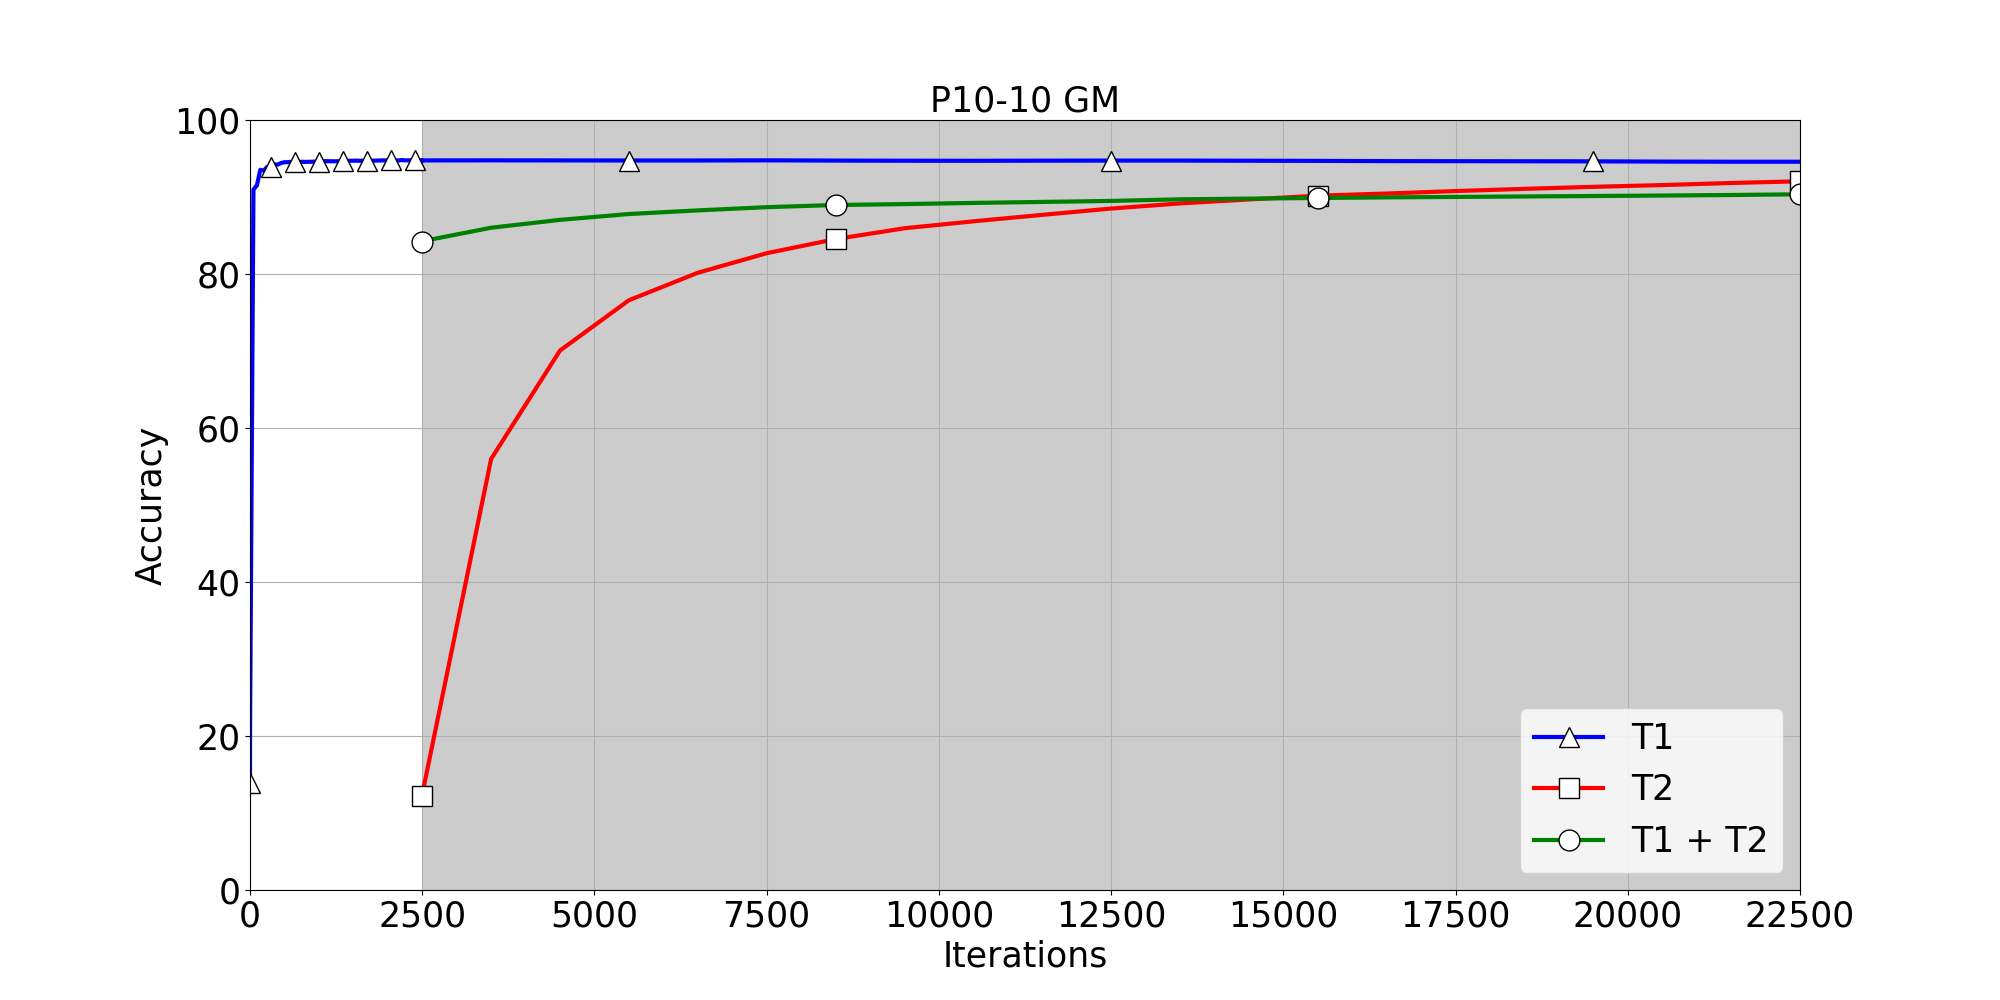
\includegraphics[width=\textwidth]{project/experiments/PM_GM}
                    \caption{EWC-GM P10-10}
                    \label{fig:ewc_gm_pm}
                \end{figure}
            \end{columns}
        \end{frame}